\documentclass[professionalfont]{beamer}
%\usecolortheme{default}
\usetheme{Madrid}
\usepackage{subcaption}
\usepackage{caption}
\usepackage{tikz-feynman,contour}
\usepackage{dsfont}

\title{\textbf{The Quantum Geometric Origin of Capacitance in Insulators}}
\subtitle{I. Komissarov, T. Holder \& R. Queiroz \\ \textit{Nat. Commun.} \textbf{15}, 4621 (2024)}

\author{Chen-Chih Wang}
\institute{NTHU}
\date{May 20, 2025}

\newcommand{\anglelr}[1]{\left\langle #1 \right\rangle}
\newcommand{\abs}[1]{\left| #1 \right|}
\newcommand{\de}{\partial}
\newcommand{\pdiff}[2]{\frac{\partial #1}{\partial #2}}
\newcommand{\diff}[2]{\frac{\mrm{d} #1}{\mrm{d} #2}}
\newcommand{\lr}[1]{\left(#1\right)}
\newcommand{\lrm}[1]{\left[#1\right]}
\newcommand{\lrg}[1]{\left\{#1\right\}}
\newcommand{\lran}[1]{\left\langle #1 \right\rangle}
\newcommand{\lra}[1]{\left|#1\right|}
\newcommand{\ket}[1]{\left| #1 \right\rangle}
\newcommand{\bra}[1]{\left\langle #1 \right|}
\newcommand{\braket}[2]{\langle #1 | #2\rangle}
\newcommand{\mrm}[1]{\mathrm{#1}}
\newcommand{\bo}[1]{\mathbf{#1}}
\newcommand{\bog}[1]{\boldsymbol{#1}}
\newcommand{\gk}{\gamma_{\mathbf{k}}}
\newcommand{\uk}{u_{\mathbf{k}}}
\newcommand{\vk}{v_{\mathbf{k}}}
\newcommand{\vkp}{v_{\mathbf{k}'}}
\newcommand{\norm}[1]{\| #1 \|}

%\setbeamercolor{frametitle}{fg=black,bg=blue}
%\setbeamertemplate{frametitle}[default][left]
%\setbeamerfont{frametitle}{size=\huge}
%\setbeamerfont{block title}{size=\Large}

%%%%%%%%%%%%%%%%%%%%%%%%%%%%%%%%%%%%%%%%%%%%%%%%

\begin{document}
\begin{frame}
    \titlepage
\end{frame}

%%%%%%%%%%%%%%%%%%  content  %%%%%%%%%%%%%%%%%%%
\begin{frame}{Content}
   \tableofcontents
% Motivations: Two questions
    % Does the quantity (capacitance $c$) depend on the quantum geometry?
    % Is $c$ a substantial contribution in quantum materials?
% Introduction
    % quantum geometry revisit
    % physical meaning (size of Wannier functions)
%  
\end{frame}
%%%%%%%%%%%%%%%%%%%%%%%%%%%%%%%%%%%%%%%%%%%%%%%%
\begin{frame}
    \begin{figure}
        \centering
        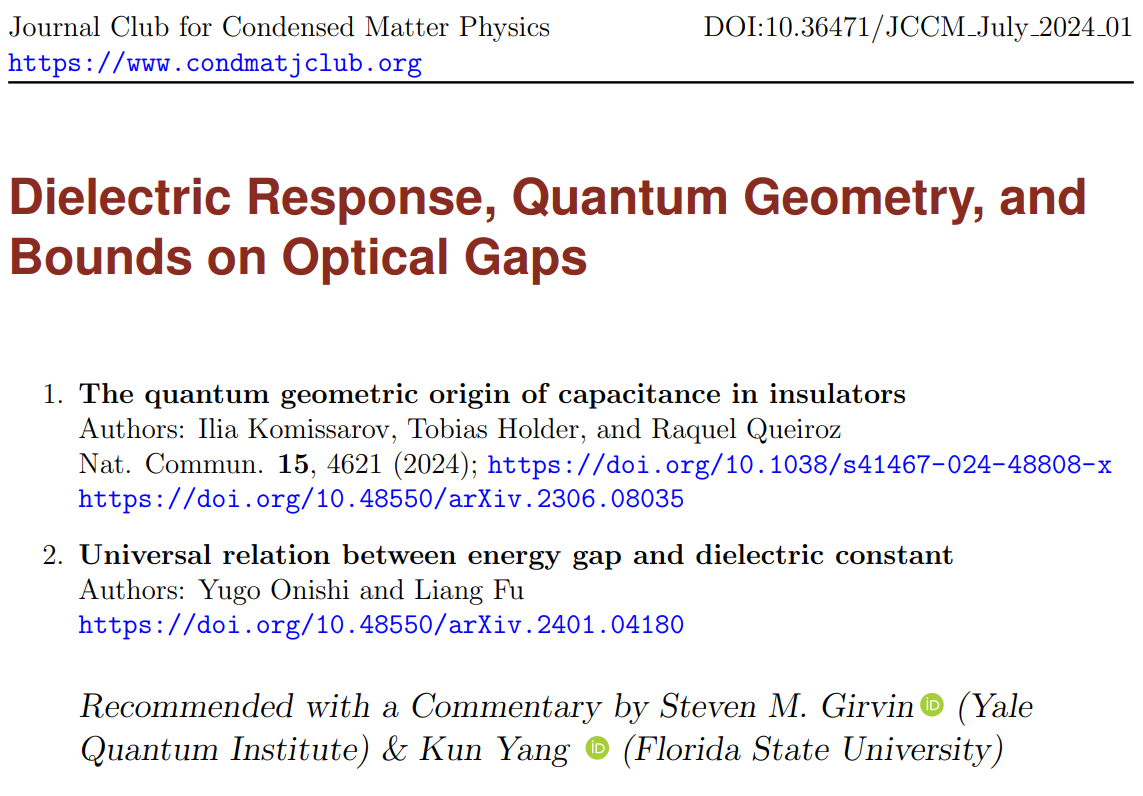
\includegraphics[width=0.8\linewidth]{article}
    \end{figure}
\end{frame}
%%%%%%%%%%%%%%%%%%%%%%%%%%%%%%%%%%%%%%%%%%%%%%%%
{
\setbeamercolor{background canvas}{bg=lightgray}
\section{Introduction}
\begin{frame}
    \centering
    \huge
    \textbf{Introduction \\ and \\ General Ideas}
\end{frame}
}
%%%%%%%%%%%%%%%%%%%%%%%%%%%%%%%%%%%%%%%%%%%%%%%%
\begin{frame}{Quantum Geometry}
\subsection{Quantum Geometry}
{\footnotesize
    Quantum geometry reflects the geometry of the Hilbert space. Here we use \textbf{momentum} as the continuous quantum number, and consider only \textbf{one band}
    \[
    \mrm{d}s^2\equiv\norm{\ket{u_n(\bo{k}+\mrm{d\bo{k}})}-\ket{u_n(\bo{k})}}^2 = \braket{\de_{k_\mu}u_n}{\de_{k_\nu}u_n}\mrm{d}k^\mu\mrm{d}k^\nu \equiv Q_{\mu\nu}\mrm{d}k^\mu\mrm{d}k^\nu
    \]
    We further impose the covariant constraint
    \[
    Q_{\mu\nu} = \braket{\de_{k_\mu}u_n}{\de_{k_\nu}u_n} \to \braket{D_{k_\mu}u_n}{D_{k_\nu}u_n} \quad;\quad D_{k_\mu}\equiv \de_{k_\mu} + iA_{\mu} ,\quad A_\mu\equiv i\braket{u_n}{\de_{k_\mu}u_n}
    \]
    Define $\mathcal{P}:=\ket{u_n}\bra{u_n}$ as the projector,
    \[
    Q_{\mu\nu} = \bra{\de_{k_\mu}u_n}\lr{\mathds{1}-\mathcal{P}}\ket{\de_{k_\nu}u_n}
    \]
    Such a tensor can be separated into real and imaginary parts,
    \[
    Q_{\mu\nu} \equiv g_{\mu\nu} + \frac{i}{2}\Omega_{\mu\nu}
    \]
    Here $g_{\mu\nu}$ is called \textit{quantum metric} and $\Omega_{\mu\nu}$ is exactly the \textit{Berry curvature}.
}

{\tiny R. Resta, Eur.Phys.J.B \textbf{79}, 121 (2011)}
\end{frame}
%%%%%%%%%%%%%%%%%%%%%%%%%%%%%%%%%%%%%%%%%%%%%%%%
\begin{frame}{Quantum Geometry}
Berry curvature:\
{\tiny
\[
\Omega_{\mu\nu} = D_{k_\mu}A_{\nu} - D_{k_\nu}A_{\mu} = i\lr{\braket{D_{k_\mu}u_n}{D_{k_\nu}u_n} - \braket{D_{k_\nu}u_n}{D_{k_\mu}u_n}} = 2\mrm{Im}\lrg{Q_{\mu\nu}}
\]
And the quantum metric is the real part,
\[
g_{\mu\nu} = \frac{Q_{\mu\nu}+Q_{\nu\mu}}{2} = \bra{u_n}r_\mu r_\nu\ket{u_n} - \bra{u_n}r_\mu\ket{u_n}\bra{u_n} r_\nu\ket{u_n}
\]
If we now consider two bands, $\mathds{1} = \ket{u_n}\bra{u_n} + \ket{u_m}\bra{u_m}$, then the formula becomes
\[
g^{\mu\nu}_{nm} =  \bra{u_n}r_\mu\ket{u_m}\bra{u_m} r_\nu\ket{u_n} \equiv r^{\mu}_{nm}r^{\nu}_{mn} = \frac{1}{2}\lr{r^{\mu}_{nm}r^{\nu}_{mn} + r^{\nu}_{nm}r^{\mu}_{mn}}
\]
With this, we can express both $g$ and $\Omega$ in multiband cases as the following
\[
    \left\{
    \begin{aligned}
    2g^{\mu\nu}_{nm} &= r^\mu_{nm}r^\nu_{mn} + r^\nu_{nm}r^\mu_{mn} \\
     -i\Omega^{\mu\nu}_{nm} &= r^\mu_{nm}r^\nu_{mn} - r^\nu_{nm}r^\mu_{mn}
    \end{aligned}
    \right.
    \]

    \textbf{Trace condition}:
    \[
    \mrm{det}Q = \mrm{det}g - \frac{\Omega^2}{4}\geq 0
    \]
    \[
    \mrm{tr}g \geq 2\sqrt{\mrm{det}g} \geq \abs{\Omega}
    \]
}

{\tiny R. Resta, Eur.Phys.J.B \textbf{79}, 121 (2011)}
\end{frame}
%%%%%%%%%%%%%%%%%%%%%%%%%%%%%%%%%%%%%%%%%%%%%%%%
\begin{frame}{Quantum Metric and Wannier Function}
\subsection{Quantum Metric and Wannier Function}
{\footnotesize
Quantum metric reflects the size of the Wannier function.
\[
\ket{u_n(\bo{k})} = \int\mrm{d}\bo{r}W_n(\bo{r})e^{-i\bo{k}\cdot \bo{r}}
\]
Thus
\[
\ket{u_n(\bo{k}+\mrm{d}\bo{k})}-\ket{u_n(\bo{k})} = \mrm{d}\bo{k}\cdot\bog{\nabla}\ket{u_n(\bo{k})} = -i\mrm{d}\bo{k}\cdot\int\mrm{d}\bo{r}W_n(\bo{r})\bo{r}e^{-i\bo{k}\cdot\bo{r}}
\]
So the infinitesimal distance is
\[
\mrm{d}s^2 = \underbrace{\lr{\int\mrm{d}\bo{r}W_n^*(\bo{r})r^\mu e^{i\bo{k}\cdot\bo{r}}}\lr{\int\mrm{d}\bo{r}W_n(\bo{r})r^\nu e^{-i\bo{k}\cdot\bo{r}}}}_{g_{\mu\nu}(\bo{k})}\mrm{d}k^\mu\mrm{d}k^\nu
\]
Therefore, the integral of quantum metric reads
\[
\int_{\mrm{BZ}}\mrm{d}\bo{k}g_{\mu\nu}(\bo{k}) = \int\mrm{d}\bo{r}\abs{W_n(\bo{r})}^2r^\mu r^\nu \equiv \anglelr{r^\mu r^\nu} 
\]
}
\end{frame}
%%%%%%%%%%%%%%%%%%%%%%%%%%%%%%%%%%%%%%%%%%%%%%%%
\begin{frame}{Conductivity and Capacitance}
\subsection{Conductivity and Capacitance}
{\footnotesize
Consider $j^\mu = \mrm{d}P^\mu/\mrm{d}t$
\[
\sigma^{\mu\nu}(\omega) = \frac{\delta j^\nu}{\delta E^\mu} = \frac{\delta}{\delta E^\mu}\left.\lr{\diff{P^\nu}{t}}\right|_{E^\mu=0}
\]
On the other hand, by linear response approach,
\begin{align*}
\sigma^{\mu\nu}\lr{\omega} &= -\frac{e^2}{h}C\epsilon^{\mu\nu} + i\omega 4\pi\chi\delta^{\mu\nu} \\
&\equiv -\frac{e^2}{h}C\epsilon^{\mu\nu} + i\omega {\color{red}c}\delta^{\mu\nu}
\end{align*}
Optical conductivity:
\[
\varepsilon(\omega) = 1+\frac{4\pi i\sigma(\omega)}{\omega} = 1+4\pi\chi(\omega)
\]}
{\large
\textbf{Motivation:}
\begin{itemize}
    \item Does the intrinsic capacitance $c$ depend on the quantum geometry?
    \item Is $c$ a substantial contribution in quantum materials?
\end{itemize}
}
\end{frame}
%%%%%%%%%%%%%%%%%%%%%%%%%%%%%%%%%%%%%%%%%%%%%%%%
\begin{frame}{Conductivity and Capacitance}
    \begin{itemize}
        \item $P^\mu$ in an insulator is determined entirely by the eigenfunctions and is related to the \textbf{Berry phase}
        {\tiny
        \[
        P^\mu = -e\anglelr{r^\mu} = -e\int_{\mrm{BZ}}\mrm{d}\bo{k}\sum_nf_n(\bo{k})\bra{u_n(\bo{k})}\hat{r}^\mu\ket{u_n(\bo{k})} = -i\hbar e\int_{\mrm{BZ}}\mrm{d}\bo{k}\sum_nf_n(\bo{k})A_n(\bo{k})
        \]
        (Note: This is the zeroth-order approximation. Later, one has to include the interaction with light.)}
        \item The definition $\frac{\delta}{\delta E^\mu}\lr{\diff{P^\nu}{t}}$ plus the Berry phase expression shows the geometric nature of the theory.
        \item Expressing the conductivity through polarization shows the direct relation between the \textbf{polarizability} and the \textbf{intrinsic capacitor}.
        
    \end{itemize}
\begin{figure}
    \centering
    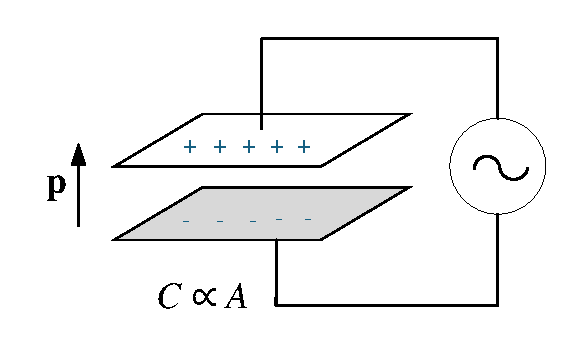
\includegraphics[width=0.4\linewidth]{Capacitor.pdf}
\end{figure}
\end{frame}
%%%%%%%%%%%%%%%%%%%%%%%%%%%%%%%%%%%%%%%%%%%%%%%%
{
\setbeamercolor{background canvas}{bg=lightgray}
\section{Methods and Results}
\begin{frame}
    \centering
    \huge
    \textbf{Methods and Results}
\end{frame}
}
%%%%%%%%%%%%%%%%%%%%%%%%%%%%%%%%%%%%%%%%%%%%%%%%
\begin{frame}{Capacitance and Quantum Metric}
\subsection{Capacitance and Quantum Metric}

{\footnotesize
    {\Large\textbf{Result:}}
    \[
    \left\{
    \begin{aligned}
    & \sigma^{\mu\nu}_{\mrm{inter}}(\omega) = -\frac{ie^2}{\hbar}\sum_{n\neq m}\int_{\mrm{BZ}}\mrm{d}\bo{k}f_{nm}\omega_{nm}\frac{r^\mu_{nm}r^\nu_{mn}}{\omega_{nm} + \omega} \\
    & \sigma^{\mu\nu}_{\mrm{intra}}(\omega) = \frac{i}{\omega}\sum_n\int_{\mrm{BZ}}f'_nJ^\mu_{nn}J^\nu_{nn}\; \Longrightarrow\text{vanishes in insulators}
    \end{aligned}
    \right.
    \]
    Consider quantum metric
    \[
    \left\{
    \begin{aligned}
    2g^{\mu\nu}_{nm} &= r^\mu_{nm}r^\nu_{mn} + r^\nu_{nm}r^\mu_{mn} \\
     -i\Omega^{\mu\nu}_{nm} &= r^\mu_{nm}r^\nu_{mn} - r^\nu_{nm}r^\mu_{mn}
    \end{aligned}
    \right.
    \]
    Eventually,
    \begin{align*}
        \sigma^{\mu\nu}_{\mrm{inter}}(\omega) &= i\omega\frac{2e^2}{\hbar}\sum_{n\neq m}\int_{\mrm{BZ}}\mrm{d}\bo{k}f_n(1-f_m)\frac{\omega_{mn}}{\omega_{mn}^2-\omega^2}g^{\mu\nu}_{nm}\\
        &\quad\quad\quad -\frac{e^2}{\hbar}\sum_{n\neq m}\int_{\mrm{BZ}}\mrm{d}\bo{k}f_n(1-f_m)\frac{\omega_{mn}^2}{\omega_{mn}^2-\omega^2}\Omega^{\mu\nu}_{nm}
    \end{align*}
  }  
\end{frame}
%%%%%%%%%%%%%%%%%%%%%%%%%%%%%%%%%%%%%%%%%%%%%%%%
\begin{frame}{Capacitance and Quantum Metric}
In the DC limit ($\omega\to 0$),
{\footnotesize
\begin{align*}
\sigma^{\mu\nu}_{\mrm{inter}}(\omega) &= -\frac{e^2}{\hbar}\underbrace{\sum_{n\neq m}\int_{\mrm{BZ}}\mrm{d}\bo{k}f_n(1-f_m)\Omega^{\mu\nu}_{nm}}_{\text{Chern number}\quad C\epsilon^{\mu\nu}}\\
&\quad\quad\quad\quad + i\omega\underbrace{\frac{2e^2}{\hbar}\sum_{n\neq m}\int_{\mrm{BZ}}\mrm{d}\bo{k}f_n(1-f_m)\frac{1}{\omega_{mn}}g^{\mu\nu}_{nm}}_{\text{Intrinsic capacitance}\quad c^{\mu\nu}}
\end{align*}
}
Then we get an important result,
\begin{equation}\label{major}
{\color{red}c^{\mu\mu}} = \frac{2e^2}{\hbar}\sum_{n\neq m}\frac{1}{\omega_{mn}}\int_{\mrm{BZ}}\mrm{d}\bo{k}f_n(1-f_m){\color{red}g^{\mu\nu}_{nm}}
\end{equation}
which bridges the \textbf{intrinsic capacitance} with the \textbf{quantum metric}.
\end{frame}
%%%%%%%%%%%%%%%%%%%%%%%%%%%%%%%%%%%%%%%%%%%%%%%%
\begin{frame}{Capacitance and Quantum Metric}
\textbf{Short Summary:}
\begin{itemize}
    \item \textbf{Multiband nature} is crucial since the intraband contribution is zero.
    \item The physical picture of the fact  $\chi \propto c\propto \int_{\mrm{BZ}}g^{\mu\nu}$ is that the more extended the wave pocket, the larger the polarizability.
    \item There is a rigorous relation between the \textbf{dielectric constant} and the \textbf{quantum metric} $\Longrightarrow$ We can use optical properties of an insulator to estimate the quantum metric.
    
\end{itemize}

\end{frame}
%%%%%%%%%%%%%%%%%%%%%%%%%%%%%%%%%%%%%%%%%%%%%%%%
\begin{frame}{Examples: Gapped Dirac Hamiltonians}
\subsection{Examples: Gapped Dirac Hamiltonians}
2D gapped Dirac Hamiltonian
\[
H = k_\mu\sigma^\mu+\frac{\Delta}{2}\sigma^z
\]
Use equation (\ref{major}), 
\[
c^{\mu\mu} = \frac{2e^2}{\hbar}\sum_{n\neq m}\frac{1}{\omega_{mn}}\int_{\mrm{BZ}}\mrm{d}\bo{k}f_n(1-f_m) g^{\mu\nu}_{nm}
\]
we have
\[
c=\mrm{tr}c^{\mu\nu} \approx \frac{2e^2}{\Delta}\int_{\mrm{BZ}}\mrm{d}\bo{k}\;\mrm{tr}g \geq \frac{e^2C}{\pi\Delta}
\]
This inequality tells us that the intrinsic capacitor diverges at a gap closing.

In this example, we can see that the \textbf{polarizability} is related to the \textbf{band gap}.

\end{frame}
%%%%%%%%%%%%%%%%%%%%%%%%%%%%%%%%%%%%%%%%%%%%%%%%
\begin{frame}{Examples: Magic Angle Twisted Bilayer Graphene}
\subsection{Examples: Magic Angle Twisted Bilayer Graphene}
TBG aligned on top of hBN. The in-plane inversion symmetry breaking leads to a gap $\Delta$.
\begin{figure}
    \centering
    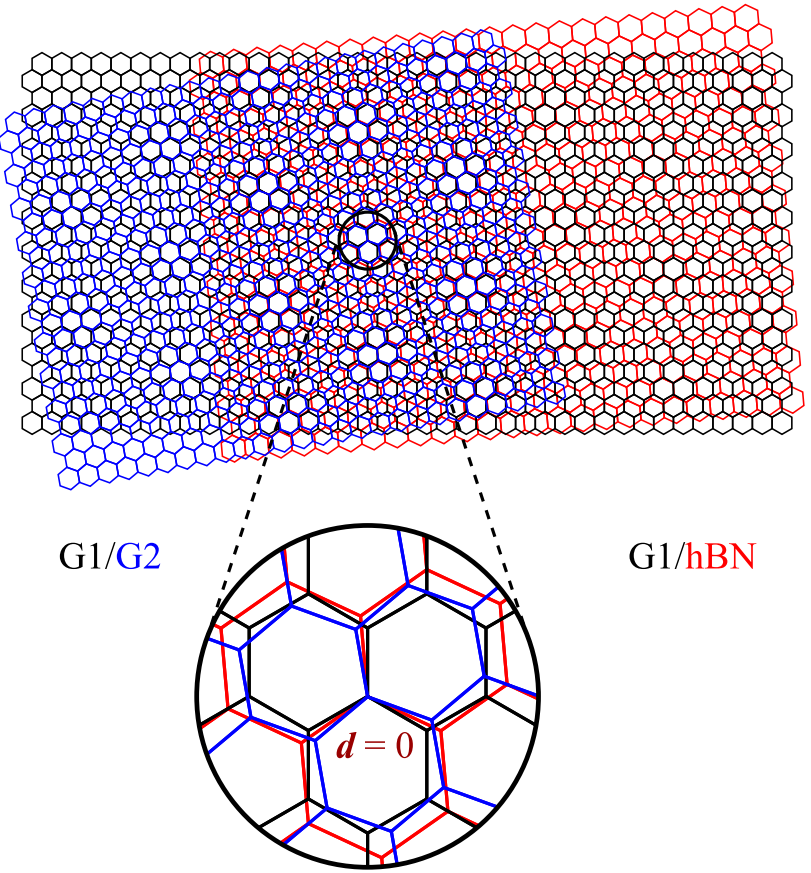
\includegraphics[height=0.5\textheight]{sheet.png}
    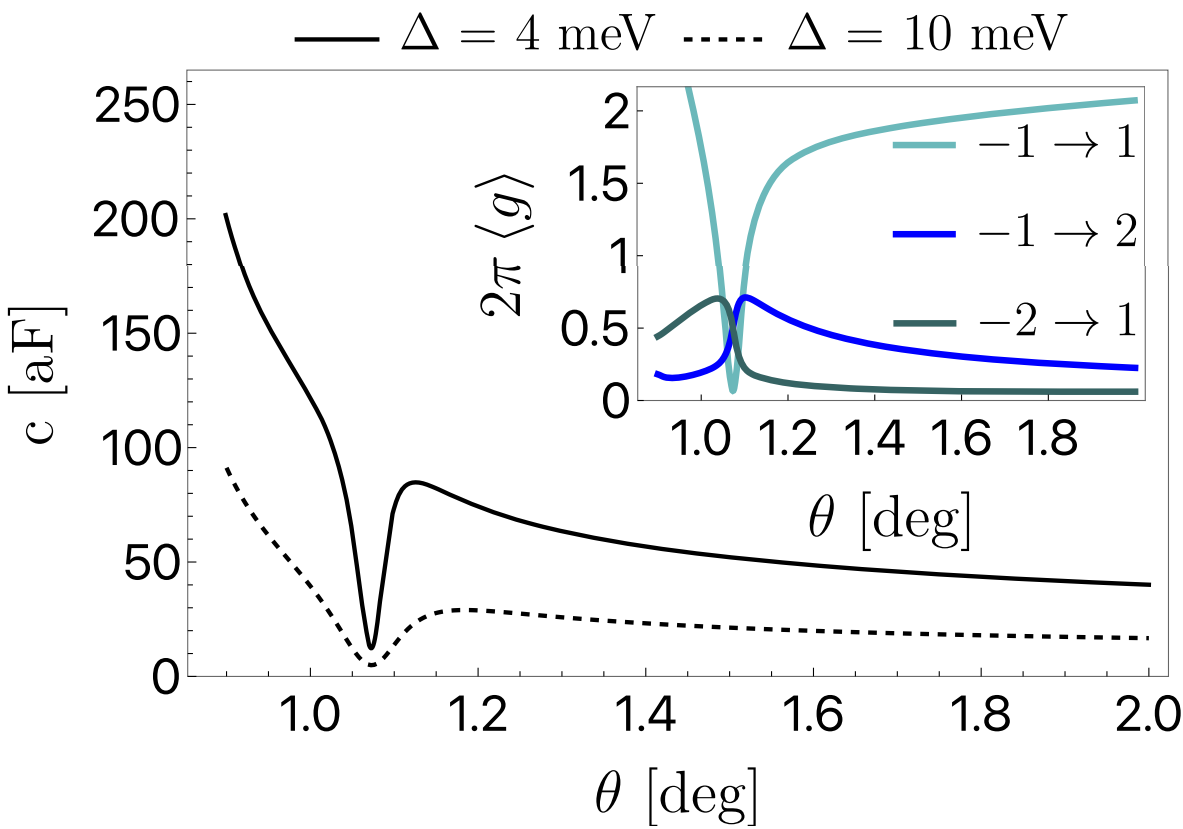
\includegraphics[height=0.5\textheight]{GrapheneMini.png}
\end{figure}
Trace condition $\mrm{tr}g\geq \abs{\Omega}/2$ is saturated at the magic angle (LLL).
\end{frame}
%%%%%%%%%%%%%%%%%%%%%%%%%%%%%%%%%%%%%%%%%%%%%%%%
\begin{frame}{Dielectric Constant and Quantum Metric}
\subsection{Dielectric Constant and Quantum Metric}
From equation (\ref{major}), the longitudinal dielectric constant is
{\footnotesize
\[
\varepsilon^{\mu\mu} = 1 + \frac{8\pi e^2}{\hbar}\sum_{n\neq m}\int_{\mrm{BZ}}\mrm{d}\bo{k}f_n(1-f_n)\frac{g_{mn}^{\mu\mu}}{\omega_{mn}} \leq 1 + \frac{8\pi e^2}{\Delta}\int_{\mrm{BZ}}\mrm{d}\bo{k}\underbrace{\sum_{n\neq m}f_n(1-f_n)g_{mn}^{\mu\mu}}_{g^{\mu\mu}}
\]
}
This is entirely contributed by electric properties.

Subsequently,
\[
\int_{\mrm{BZ}}\mrm{d}\bo{k}\;\mrm{tr}g   \geq  \frac{\Delta}{8\pi e^2}(\varepsilon-1)
\]
In this perspective, we can estimate the quantum metric from the experimental values of \textbf{dielectric constant $\varepsilon$} and \textbf{band gap $\Delta$}.
\end{frame}
%%%%%%%%%%%%%%%%%%%%%%%%%%%%%%%%%%%%%%%%%%%%%%%%
\begin{frame}{Dielectric Constant and Quantum Metric}
\begin{figure}
    \centering
    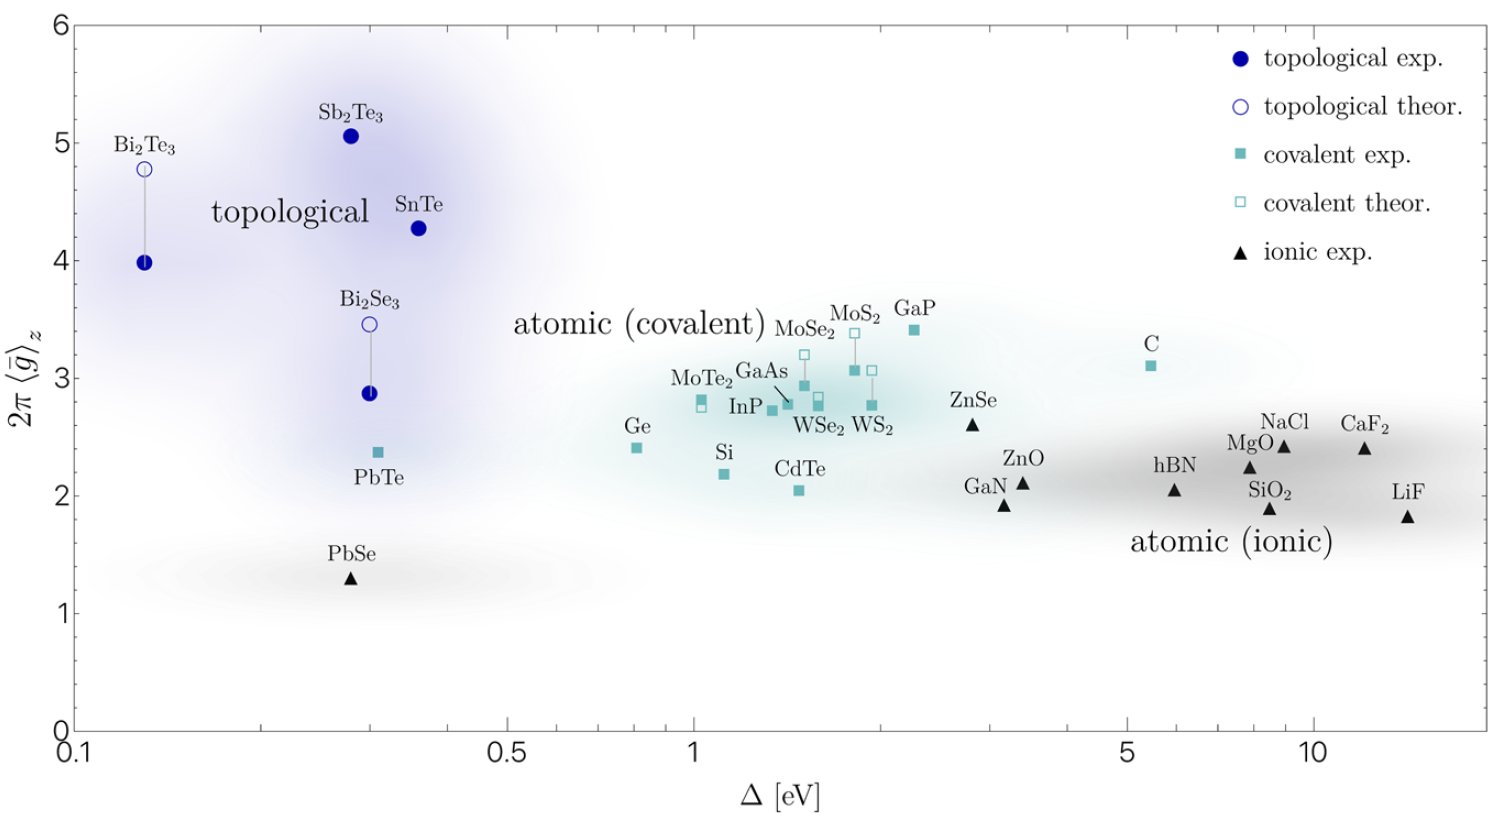
\includegraphics[width=0.8\linewidth]{experiment.png}
\end{figure}
{\footnotesize\[
{\color{red}\anglelr{g}_z}\equiv \int\frac{a_z\mrm{d}k_z}{2\pi}\int\frac{\mrm{d}^2\bo{k}}{(2\pi)^2}(g^{xx} + g^{yy}){\color{red}\geq} \frac{4\pi}{e^2}a_z\Delta\lr{\varepsilon-1} \equiv {\color{red}\anglelr{\bar{g}}_z}
\]}
\end{frame}
%%%%%%%%%%%%%%%%%%%%%%%%%%%%%%%%%%%%%%%%%%%%%%%%
\begin{frame}{Conclusion}
\section{Conclusion}
\begin{itemize}
    \item The relation between conductivity in insulators and the quantum metric is established.
    \item In insulators, both the \textbf{polarizability} and the \textbf{conductivity} are completely determined by the properties of the Hilbert space (quantum geometry)
    \item Optical properties such as $\varepsilon$ could be used to estimate the quantum metric.
\end{itemize}
\end{frame}
%%%%%%%%%%%%%%%%%%%%%%%%%%%%%%%%%%%%%%%%%%%%%%%%
\begin{frame}{Outlook}
    \section{Outlook}

    {\footnotesize
    \textbf{Quantum Weight} (Y.Onishi \& L.Fu, arXiv:2406.06783v3)
    The quantum metric is intimately related to the structure factor (number fluctuation)
    \[
    S_\bo{q}\equiv \frac{1}{V}\anglelr{\hat{n}_\bo{q}\hat{n}_{-\bo{q}}} \approx \frac{1}{2\pi}K_{\alpha\beta}q^\alpha q^\beta
    \]
    where $K_{\alpha\beta}$ is called \textit{Quantum Weight}. It has a relation 
    \[
    K_{\mu\nu} = 2\pi\int_{\mrm{BZ}}\frac{\mrm{d}^D\bo{k}}{(2\pi)^D}g^{\mu\nu}(\bo{k})
    \]
    (Which is related to $\chi \propto \anglelr{\rho(r)\rho(r')}$ from the perspecive provided by Fluctuation Dissipation Theorem) 
    
    At the same time, the entanglement entropy also has things to do with number correlation (G.C.Levine \textit{et al}. PRA \textbf{83}, 013623 (2011))
    \[\int\mrm{d}r\mrm{d}r'\anglelr{n(r)n(r')}\propto S\]
    So it is promising to build a connection between \textbf{quantum entanglement} and \textbf{quantum geometry}.
    }
    
\end{frame}


\end{document}